\documentclass[10pt,twocolumn,letterpaper]{article}

\usepackage{times}
\usepackage{graphicx}
\usepackage{float}
\usepackage[italian]{babel}
\usepackage{csvsimple}
\usepackage[shortlabels]{enumitem}
\usepackage{listings}

\begin{document}


\title{Random Maze Solver\\
\large Parallel Programming for Machine Learning}

\author{Sofia Galante\\
\small sofia.galante@stud.unifi.it\\
}
\date{}
\maketitle
\thispagestyle{empty}

\section{Introduzione}

Il programma scritto per questo esperimento è un \textbf{Random Maze Solver}: un labirinto (generato in modo random) viene risolto da delle particelle che si muovono al suo interno, scegliendo il percorso da seguire randomicamente.\\
La particella più veloce (cioè che esce dal labirinto con il minor numero di passi) mostra il cammino corretto da seguire all'interno del labirinto.\\
Si sono creati due diversi \textbf{Random Maze Solver}: uno di tipo sequenziale (in cui cioè le particelle entrano nel labirinto una per volta) e uno di tipo parallelo (in cui più particelle risolvono il labirinto contemporaneamente).\\
\\
Lo scopo di questo elaborato è quello di osservare lo \textit{speedup} ottenuto nel secondo tipo di \textbf{Random Maze Solver} rispetto al primo.\\
Il linguaggio di programmazione utilizzato è il C++ (con compiler MinGW) e la parallelizzazione è stata svolta con \textbf{OpenMP}.\\
\\
Gli esperimenti si sono svolti su un PC con Windows 10 come sistema operativo e una CPU Intel Core i5-11400.

\section{Organizzazione del codice}
\begin{figure}[H]
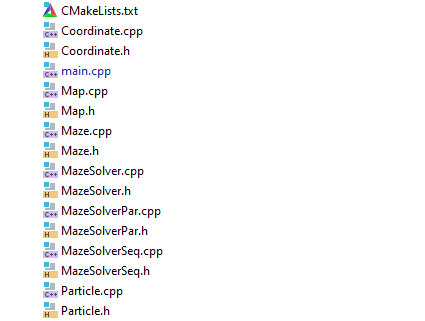
\includegraphics[width=1\linewidth]{code/org.png}
\caption{\small Organizzazione del codice}
\label{organizzazione}
\end{figure}
Il codice è composto da più file.\\
Il file \textbf{main.cpp} contiene tutte le funzioni relative ai test da svolgere e la funzione \textit{main()} del programma; si noti che quest'ultima riceve dall'esterno il nome del file con cui salvare i test svolti.\\
Gli altri file contengono le 7 classi utilizzate dal programma.

\subsection{La classe \textit{Coordinate} e la classe \textit{Map}}
La classe \textbf{Coordinate} serve a indicare la coordinata di una posizione nel labirinto. Essa permette di settare le coordinate di un punto (con il metodo \textit{setCoordinate()}) e di osservare se due punti hanno le stesse coordinate o no (con un override degli operatori \textit{==} e \textit{!=}).\\
\\
La classe \textbf{Map} rappresenta la mappa del labirinto. Essa viene usata dalla classe \textbf{Maze} per definire quali coordinate del labirinto siano muri o meno e quale direzione sia stata presa nella creazione del cammino da una cella all'altra e dalla classe \textbf{Particle} per tenere traccia dei movimenti fatti all'interno del labirinto.

\subsection{La classe \textit{Maze}}
La classe \textbf{Maze} rappresenta il labirinto da risolvere. Quando viene creato un oggetto da questa classe, il costruttore procede alla costruzione randomica del labirinto, facendo in modo che esista sempre un cammino valido che vada dall'entrata all'uscita (anche queste sono scelte randomicamente su due mura opposte).\\
I metodi che vengono utilizzati nella creazione del labirinto sono:
\begin{enumerate}
\item{il metodo \textit{createMaze()} che coordina la creazione del labirinto, partendo dalla creazione di un cammino valido e poi riempiendo il resto del labirinto con cammini aggiuntivi;}
\item{i metodi \textit{setStartAndEnd()} e \textit{setStartOrEnd()} che scelgono randomicamente l'entrata e l'uscita del labirinto;}
\item{i metodi \textit{placeWalls()} e \textit{placeWall()} che inseriscono i muri nel labirinto;}
\item{i metodi \textit{validMoves()} e \textit{isPointValid()} che servono a trovare le mosse valide da compiere per continuare a costruire il cammino nel labirinto;}
\item{il metodo \textit{getDirection()} che scrive nella coordinata corrente la direzione da cui è stata scelta quella coordinata;}
\item{il metodo \textit{rewind()} che torna indietro nel cammino se ci si trova in un vicolo cieco, in modo da deviare il percorso per cercare l'uscita;}
\item{il metodo \textit{recovery()} che viene attivato solo nel momento in cui i muri siano stati posizionati in modo tale da rendere impossibile raggiungere l'uscita; in questo caso si riparte dall'uscita e si inizia a creare un cammino per poi abbattere il primo muro che si trova con il metodo \textit{findWallsToRemove()}; si continua finché non si congiunge l'uscita con l'entrata.}
\end{enumerate}
Durante la creazione del labirinto si decide anche un numero massimo di passi con cui le particelle devono risolverlo.

\subsection{La classe \textit{Particle}}
La classe \textbf{Particle} rappresenta le particelle che devono risolvere il labirinto. Ogni istanza di questa classe mantiene nel suo stato il numero di passi fatti e il percorso intrapreso dall'entrata all'uscita.

\subsection{Le classi \textit{MazeSolver}, \textit{MazeSolverSeq} e \textit{MazeSolverPar}}
La classe \textbf{MazeSolver} contiene al suo interno i metodi che servono a far muovere le particelle nel labirinto. Il MazeSolver tiene traccia della posizione della particella e sceglie quale mossa farle compiere in modo randomico, escludendo le mosse in cui essa andrebbe in una posizione occupata da un muro. Inoltre controlla anche che la particella non superi i numeri di passi massimi per la soluzione del labirinto. Infine stampa a schermo il percorso seguito dalla particella più veloce.\\
Uno dei metodi di questa classe, \textit{solve()}, è un metodo puramente virtuale.\\
Le classe \textbf{MazeSolverSeq} e \textbf{MazeSolverPar} sono classi derivate da \textbf{MazeSolver}. Esse implementano in modo diverso il metodo \textit{solve()} così da crearne una versione sequenziale e una parallela. Questo metodo è responsabile della creazione delle particelle, dell'inizio del loro movimento nel labirinto e della scelta della particella vincitrice (cioè quella che esce più velocemente dal labirinto).\\
La parallelizzazione di questo metodo viene descritta nel dettaglio nella sezione successiva.\\
Si noti che la classe \textbf{MazeSolverPar} crea anche una versione parallela del metodo responsabile per la scelta delle mosse valide. Questa versione prevede l'utilizzo di un \textbf{lock} ed è stata utilizzata per svolgere uno dei test presenti nella sezione 4.

\section{Parallelizzazione compiuta in \textit{MazeSolverPar}}
Il codice di soluzione del labirinto è stato parallelizzato in due punti: nella risoluzione del labirinto da parte delle particelle e nella scelta della particella vincitrice.

\subsection{Parallelizzazione della risoluzione del labirinto da parte delle particelle}
\begin{figure}[H]
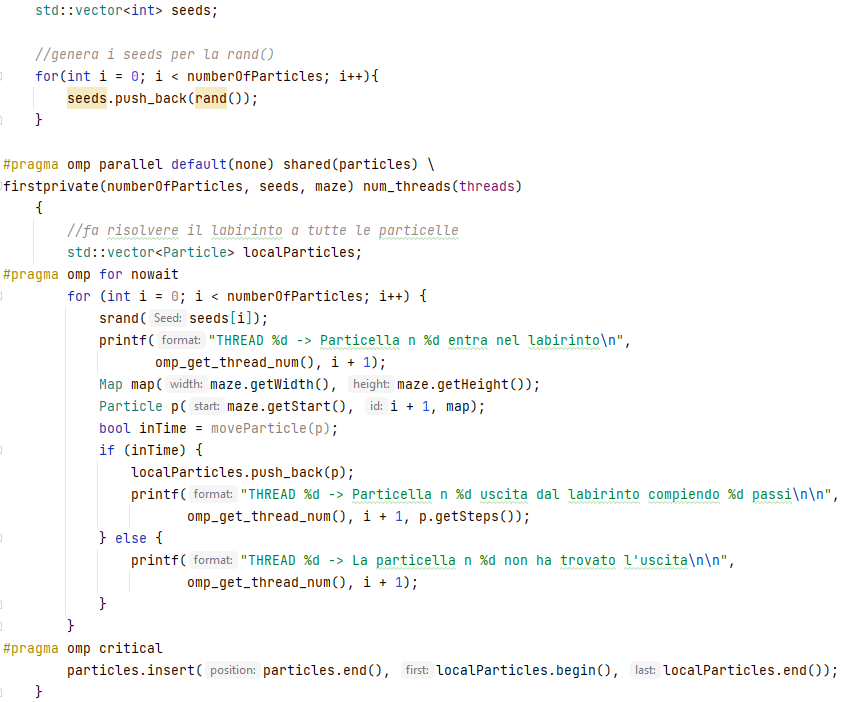
\includegraphics[width=1\linewidth]{code/par1.png}
\caption{\small Parallelizzazione della risoluzione del labirinto da parte delle particelle}
\label{par1}
\end{figure}
Per parallelizzare la creazione delle particelle e la loro risoluzione del labirinto, è stata creata una sezione \textit{omp parallel}. Essa è divisa in due parti:
\begin{enumerate}
\item{una sezione \textit{omp for} nella quale i thread generano e gestiscono in parallelo le particelle, salvando in un vettore locale (\textbf{localParticles}) le particelle che escono dal labirinto in tempo (cioè non compiendo più passi di quelli massimi); questa sezione è marcata con una \textit{nowait}, in quanto non è richiesto che i thread si aspettino a vicenda prima di passare alla fase successiva;}
\item{una sezione \textit{omp critical} in cui il contenuto dei vettori locali viene inserito in una variabile shared (\textbf{particles}).}
\end{enumerate}
Per fare in modo che le particelle utilizzassero una sequenza randomica per il movimento differente le une dalle altre, si è generato un \textit{seed} per ogni particella. Questi sono stati salvati all'interno di un vettore.\\
Per diminuire il più possibile gli accessi in memoria, le variabili \textbf{numParticles} (numero di particelle da creare), \textbf{seeds} (vettore contenente i seed per la generazione dei numeri random) e \textbf{maze} (il labirinto da risolvere) sono stati marcati come \textit{firstprivate}, in modo tale che ogni thread ottenesse una versione privata della variabile inizializzata al valore scelto prima della parallelizzazione.

\subsection{Parallelizzazione della scelta della particella vincitrice}
\begin{figure}[H]
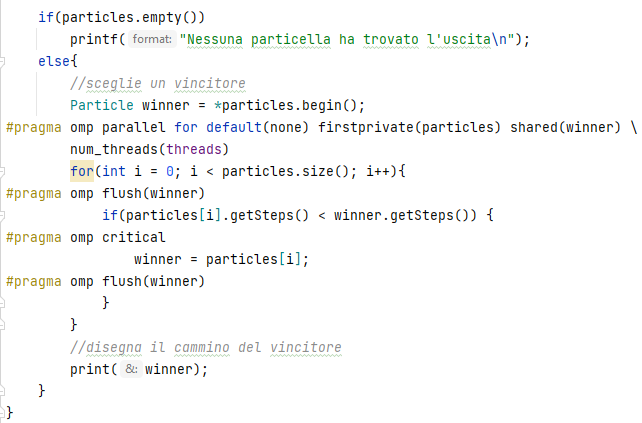
\includegraphics[width=1\linewidth]{code/par2.png}
\caption{\small Parallelizzazione della scelta della particella vincitrice}
\label{par2}
\end{figure}
Per scegliere il vincitore si è compiuta una ricerca della particella con il minor numero di passi in modo parallelo all'interno del vettore \textbf{particles}.\\
Per la parallelizzazione si è utilizzato un \textit{omp parallel for}.\\
Visto che la variabile \textbf{winner} (corrispondente alla particella vincente) è \textit{shared}, il suo accesso in scrittura è stato marcato come \textit{critical} e un \textit{flush} della variabile viene effettuato sia prima della lettura che dopo la scrittura, in modo tale che tutti i thread possano accedere al valore aggiornato.\\
L'altra variabile utilizzata (\textbf{particles}) è stata invece marcata come \textit{firstprivate}.

\section{Esperimenti svolti e risultati}
Per osservare lo \textit{speedup} ottenuto dalla parallelizzazione del codice si sono compiuti diversi esperimenti.\\
In ognuno di essi si è generato il labirinto e si è fatto risolvere sia da un \textbf{MazeSolverSeq} sia da un \textbf{MazeSolverPar}, mettendone poi a confronto i tempi di esecuzione al variare:
\begin{enumerate}
\item{della dimensione del labirinto;}
\item{del numero di particelle;}
\item{del numero di thread generati nella versione parallela.}
\end{enumerate}
Infine si è anche compiuto un esperimento andando a osservare come l'inserimento di un \textit{lock} rallentasse enormemente l'esecuzione del programma.\\
\\
Tutti gli esperimenti sono stati lanciati dal programma python \textbf{tests.py}. Ogni esperimento è stato svolto 10 volte. I risultati sono stati ottenuti facendo la media del tempo di esecuzione di ogni run (dopo aver eliminato i tempi massimi e minimi ottenuti). Tutti i risultati (sia quelli delle singole iterazioni dei test, sia quelli finali) sono salvati in appositi file csv.\\
Il programma ha anche generato i grafici riportati in seguito. 

\subsection{Variazione della dimensione del labirinto}

Il primo test svolto osserva come varia il tempo impiegato dai due metodi di risoluzione all'aumentare della dimensione del labirinto.\\
Il valore dei parametri di interesse è:
\begin{enumerate}[-]
\item{numero di particelle = 50;}
\item{numero di thread per la versione parallela = 10;}
\item{dimensioni del labirinto che partono da 5x5 e arrivano fino a 100x100.}
\end{enumerate}

\begin{figure}[H]
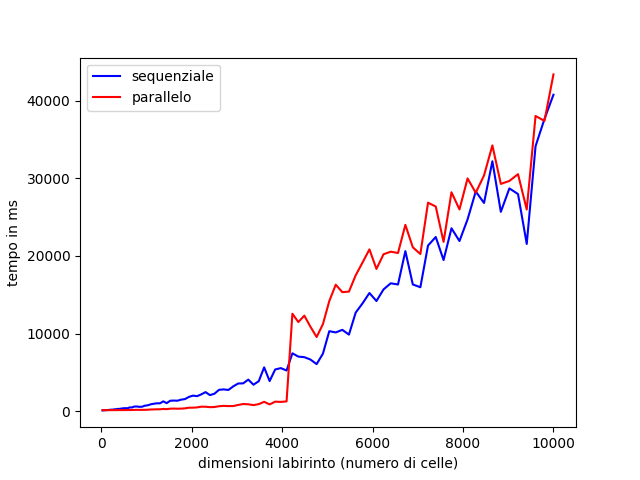
\includegraphics[width=1.1\linewidth]{test/dimTest/result.png}
\caption{\small Tempo impiegato dalla risoluzione sequenziale e dalla risoluzione parallela del labirinto al variare della dimensione (50 particelle).}
\label{t1}
\end{figure}

Questo primo test mostra come l'aumento della dimensione del labirinto possa causare un rallentamento della versione parallela del solver rispetto alla versione sequenziale.\\
Si ipotizza che questo rallentamento possa avvenire per un problema di memoria: la cache della CPU non è in grado di mantenere memorizzate le \textit{Map} di ogni \textit{Particle}, causando lo swap di queste e quindi un rallentamento del tempo di esecuzione.\\
Per vedere se il problema può essere questo, si è svolto nuovamente il test precedente ma utilizzando 2 diversi \textbf{Maze Solver paralleli}, ognuno con un differente numero di threads (2 e 10).\\
Il test in questione parte da una dimensione di 50x50 e arriva fino alla dimensione di 100x100, aumentando il lato di 5 in 5. Il motivo per cui si parte da una dimensione più alta della precedente è perché, guardando il grafico, si nota che la dimensione considerata "troppo grande" è oltre 4000, quindi valori troppo piccoli sono inutili per questo esperimento.\\
Il risultato ottenuto è il seguente:

\begin{figure}[H]
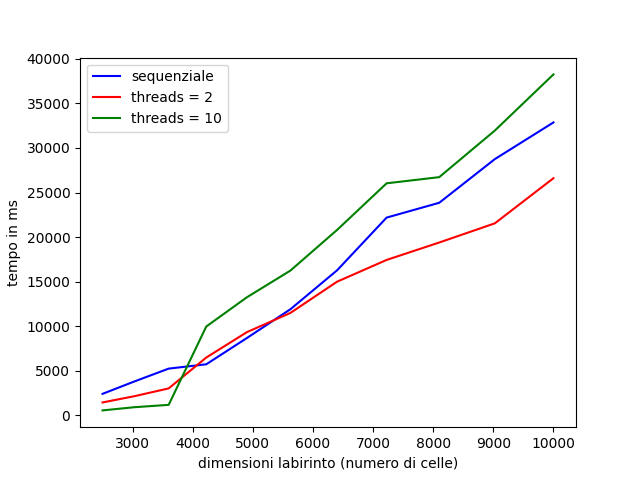
\includegraphics[width=1.1\linewidth]{test/dimTestV2/result.png}
\caption{\small Tempo impiegato dalla risoluzione sequenziale e da 4 risoluzioni parallele del labirinto al variare della dimensione (50 particelle).}
\label{t1_2}
\end{figure}

Come possiamo osservare da questo risultato, la velocità di esecuzione per soli due thread resta maggiore (tranne che per un tratto) della velocità sequenziale, facendo pensare che l'intuizione avuta sia giusta. Inoltre, il tratto in cui il tempo di esecuzione aumenta potrebbe essere spiegato dal fatto che ci siano problemi di memoria anche per soli due thread ma, superata una certa dimensione (guardando il grafico, intorno a 5500), il tempo impiegato per la gestione della memoria non è così alto da rendere il tempo di esecuzione maggiore di quello dell'algoritmo sequenziale.

\subsection{Variazione del numero di particelle}

Questo test osserva come variano i tempi all'aumentare del numero di particelle.\\
Il valore dei parametri di interesse è:
\begin{enumerate}[-]
\item{numero di particelle che varia da 1 a 501, aumentando di 10 in 10 (100 iterazioni in totale);}
\item{numero di thread per la versione parallela = 10;}
\item{dimensioni del labirinto = 50x50}
\end{enumerate}

\begin{figure}[H]
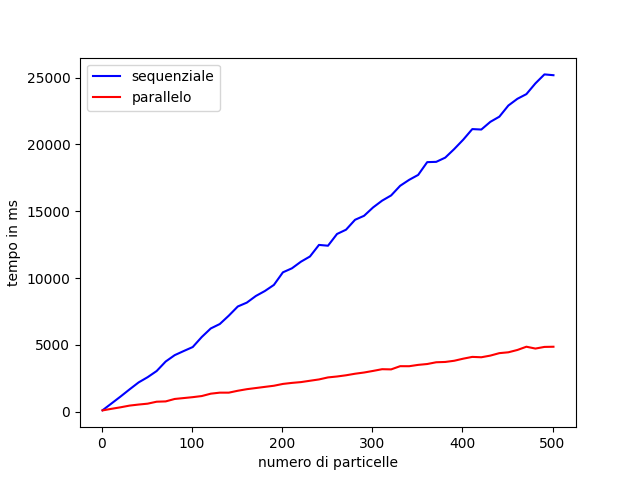
\includegraphics[width=1.1\linewidth]{test/particlesTest/result.png}
\caption{\small Tempo impiegato dalla risoluzione sequenziale e dalla risoluzione parallela del labirinto al variare del numero di particelle.}
\label{t2}
\end{figure}

Come si può osservare, maggiore è il numero di particelle, maggiore è la differenza nei tempi di esecuzione del programma.\\
Questo risultato mette in luce quanto l'utilizzo della versione parallela sia utile nel caso in cui ci siano molte particelle da far muovere all'interno del labirinto.\\
In questo caso, infatti, anche se vi fosse un rallentamento dovuto alla cache, si vede che il tempo di esecuzione dell'algoritmo sequenziale resta nettamente superiore a quello dell'algoritmo parallelo.

\subsection{Variazione del numero di thread}

In questo test viene variato il numero di thread utilizzati dall'algoritmo parallelo. Si noti che il test sequenziale viene svolto una volta sola, in quanto nessun suo parametro viene modificato.\\
Il valore dei parametri di interesse è:
\begin{enumerate}[-]
\item{numero di particelle = 500;}
\item{numero di thread che aumenta da 1 a 100;}
\item{dimensioni del labirinto = 50x50}
\end{enumerate}

\begin{figure}[H]
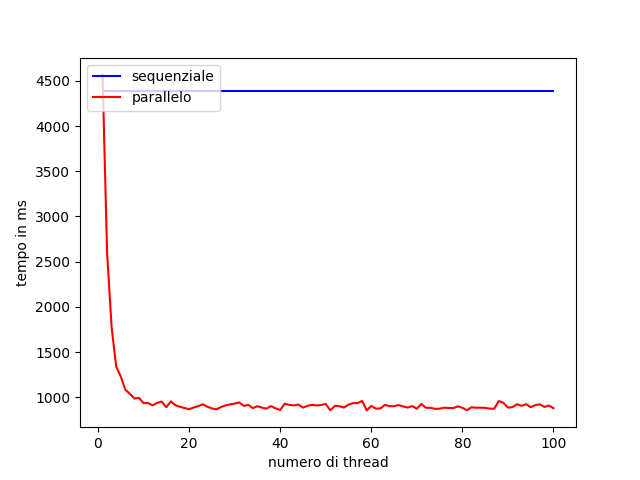
\includegraphics[width=1.1\linewidth]{test/threadsTest/result.png}
\caption{\small Tempo impiegato dalla risoluzione sequenziale e dalla risoluzione parallela del labirinto al variare del numero dei thread.}
\label{t3}
\end{figure}

Come si può osservare dal grafico il metodo parallelo è sempre migliore di quello sequenziale, ma, una volta raggiunto un certo numero di thread, il tempo di esecuzione sembra stabilizzarsi.\\
Questo fatto mostra come si raggiunga una soglia in cui l'aumento dei thread diventa inutile per la velocizzazione ulteriore del programma: il tempo impiegato a gestire quel numero dei thread è maggiore del tempo guadagnato dalla divisione del lavoro in quegli stessi thread.\\
Per avere un'ulteriore prova di ciò, si è deciso di fare una seconda versione dell'esperimento. In questo caso si è considerato tre diversi risolutori paralleli: il primo solver utilizza 10 thread, il secondo 100 e il terzo 1000.\\
Tutti e tre i solver fanno risolvere un labirinto di dimensioni 50x50 a un numero di particelle variabile da 1 a 1001 (il numero di particelle viene aumentato di 100 in 100, per un totale di 10 iterazioni).\\

\begin{figure}[H]
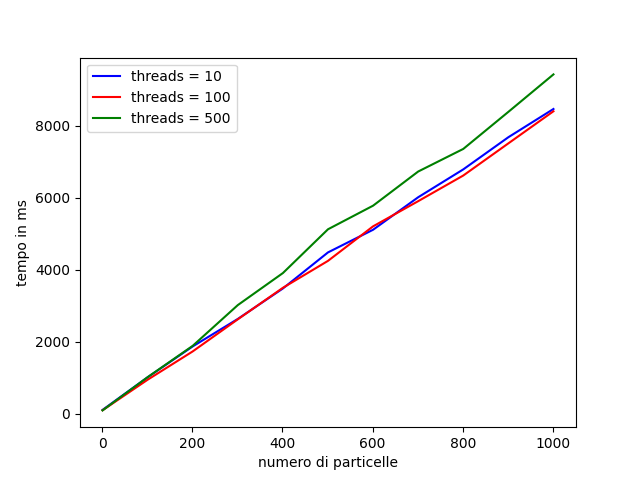
\includegraphics[width=1.1\linewidth]{test/threadsTestV2/result.png} 
\caption{\small Tempo impiegato da 3 diverse risoluzioni parallele con diverso numero di thread al variare del numero di particelle.}
\label{t3_2}
\end{figure}

Il risultato di questo secondo test ci mostra come le supposizioni fatte in quello precedente siano corrette: nonostante le particelle aumentino fino ad arrivare a 1001, il tempo di esecuzione del solver che utilizza 500 thread è maggiore dei solver che utilizzano 100 e 10 thread.\\
Inoltre la differenza tra gli altri due solver è molto sottile, dimostrando come anche solo una parallelizzazione compiuta da 10 thread sia sufficiente a ottenere uno \textit{speedup} più che buono.\\
\\
Questo fatto può essere spiegato osservando che più i thread aumentano, più aumenta il tempo per la loro gestione: nel caso in cui si abbiano 100 thread, il tempo riservato alla loro gestione viene bilanciato dalla diminuzione del tempo di esecuzione dell'algoritmo, portando questa esecuzione ad avere una velocità simile a quella svolta con 10 thread; nel caso dei 500 thread, invece, il tempo per la gestione dei thread è troppo grande e, quindi, lo speedup ottenuto dall'esecuzione del programma non basta per bilanciarlo (si va in overhead).

\subsection{Inserimento del lock}

Questo ultimo test è stato svolto per mostrare come l'inserimento di un lock possa andare a rallentare enormemente il tempo di esecuzione parallelo, rendendolo anche (molto) più lento della versione sequenziale.\\
Il lock in questione è stato inserito nella scelta delle mosse valide per la particella. Ogni volta che il MazeSolver deve scegliere le mosse possibili, infatti, esso controlla se la particella può muoversi nelle quattro direzioni intorno al punto in cui si trova e, se può farlo, inserisce la mossa nel vettore di mosse possibili. Inserendo una parallelizzazione a questo livello, si voleva fare in modo che quattro diversi thread controllassero le quattro mosse.\\
Il lock è stato inserito per la scrittura delle mosse possibili nel vettore.\begin{figure}[H]
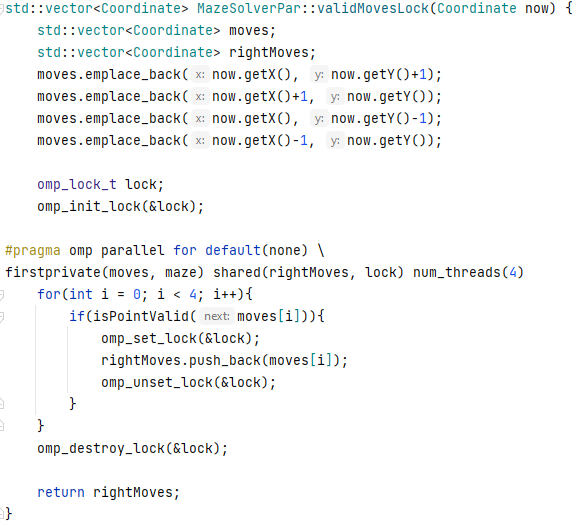
\includegraphics[width=1\linewidth]{code/lock.png} 
\caption{\small Inserimento del lock.}
\label{lock}
\end{figure}
Il valore dei parametri in questo caso è:
\begin{enumerate}[-]
\item{numero di particelle = 10;}
\item{numero di thread = 10;}
\item{dimensioni del labirinto = 20x20}
\end{enumerate}
Il risultato dei tempi impiegati è il seguente:
\begin{table}[H]
\csvautotabular[separator=semicolon]{test/lockTest/result.csv}
\caption{Variazione del tempo di esecuzione con l'inserimento del lock}
\label{t4}
\end{table}
Come si può osservare il tempo impiegato dalla versione parallela con il lock non solo è maggiore del tempo parallelo senza lock, ma è nettamente superiore anche al tempo sequenziale.\\
Questa enorme differenza nei tempi è data dalla gestione del lock da parte del sistema che impiega, quindi, un tempo decisamente maggiore di quello guadagnato dalla parellilazione della scelta della mossa possibile.\\
\\
Inoltre, un ulteriore rallentamento è dato anche dall'aumento dei thread: i thread nel ciclo for esterno (quello della creazione e gestione delle particelle) attivano quattro thread per uno, causando un aumento elevato del numero di thread totali.\\
Per questi motivi, quel livello di parallelizzazione e il lock devono essere eliminati.
\end{document}
